\chapter{Microtubule Structure \& Function}
\label{ch:microtubule-structure-function}

\begin{nontechnical}
\textbf{Microtubules are the ``scaffolding'' of your cells}---tiny hollow tubes made of proteins that give cells their shape and move things around. They're incredibly small: 25 nanometers wide (1/4000th the width of a human hair).

\textbf{What they definitely do:}
\begin{itemize}
\item \textbf{Structural support:} Like steel beams, they keep cells rigid
\item \textbf{Transportation highways:} Roads for ``molecular trucks'' (motor proteins)
\item \textbf{Cell division:} Pull chromosomes apart during cell division
\item \textbf{Movement:} Form the core of sperm tails and lung cilia
\end{itemize}

\textbf{The quantum controversy:} Some scientists propose that microtubules in brain cells might use quantum mechanics to process information or even generate consciousness. This is \emph{highly speculative}---most neuroscientists are skeptical because brains are too warm and wet for quantum effects (which usually need extreme cold and isolation).

\textbf{Current status:} Microtubules are essential for cell function (proven). Whether they do anything quantum-related in the brain remains an open question requiring better experiments.
\end{nontechnical}

\section{Overview}
\label{sec:overview}

\textbf{Microtubules} are cylindrical protein polymers that form part of the cytoskeleton in eukaryotic cells. Beyond their established structural and transport roles, microtubules have been proposed as substrates for quantum information processing in neurons---a highly speculative hypothesis that remains controversial.

\begin{keyconcept}
Microtubules are hollow protein cylinders with an outer diameter of \textbf{25~nm}, composed of 13 protofilaments arranged in a helical lattice. They exhibit \textbf{dynamic instability}, stochastically switching between growth and rapid shrinkage, enabling rapid reorganization of the cellular cytoskeleton.
\end{keyconcept}

\textbf{Established roles}:
\begin{itemize}
\item Structural support (cell shape, mechanical rigidity)
\item Intracellular transport (motor protein tracks)
\item Cell division (mitotic spindle)
\item Cilia and flagella (motility)
\end{itemize}

\textbf{Speculative roles}:
\begin{itemize}
\item Quantum computation in neurons
\item Consciousness substrates (Orch-OR theory)
\item Information integration beyond classical networks
\end{itemize}

\section{Molecular Structure}
\label{sec:molecular-structure}

\subsection{Tubulin Dimers}
\label{subsec:tubulin-dimers}

\textbf{Basic unit}: $\alpha$-$\beta$ tubulin heterodimer
\begin{itemize}
\item \textbf{$\alpha$-tubulin}: 451 amino acids, $\sim$50~kDa, globular protein
\item \textbf{$\beta$-tubulin}: 445 amino acids, $\sim$50~kDa, globular protein
\item \textbf{Dimer}: 8~nm long, 4~nm diameter
\item \textbf{GTP binding}: Both subunits have GTP-binding sites; $\beta$-tubulin is hydrolysis-active
\end{itemize}

\textbf{Key structural features}:
\begin{itemize}
\item \textbf{Aromatic residues}: 16~Trp, 25~Tyr, 39~Phe per dimer (potential quantum chromophores)
\item \textbf{Hydrophobic core}: Stabilizes folded structure
\item \textbf{C-terminal tail}: Acidic, flexible, extends from surface ($\sim$15 amino acids)
\end{itemize}

\textbf{Crystal structure}: Resolved to 3.5~Å (Nogales et al., 1998)

\subsection{Protofilaments and Lattice Structure}
\label{subsec:protofilaments-lattice}

\textbf{Assembly}:
\begin{itemize}
\item Tubulin dimers polymerize head-to-tail $\rightarrow$ \textbf{protofilament}
\item 13 protofilaments associate laterally $\rightarrow$ cylindrical microtubule
\item Outer diameter: \textbf{25~nm}
\item Inner diameter: \textbf{15~nm}
\item Wall thickness: \textbf{5~nm}
\end{itemize}

\begin{center}
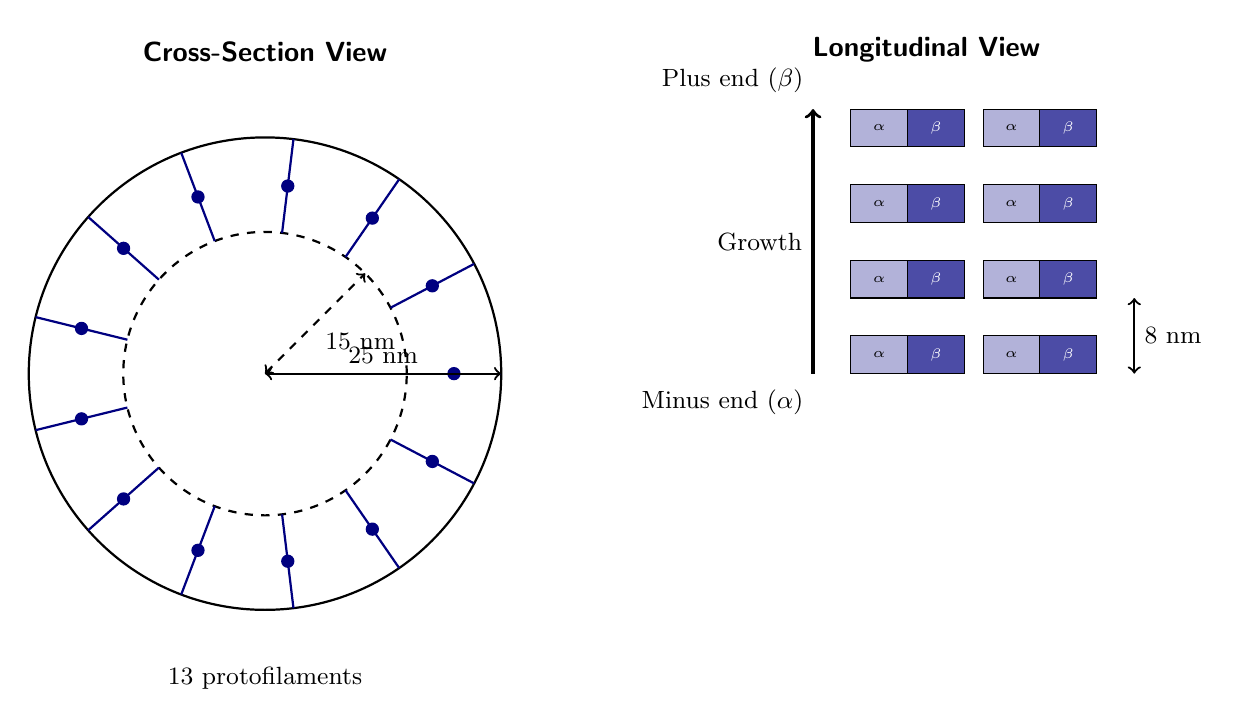
\begin{tikzpicture}[scale=1.2]
% Draw cylindrical microtubule structure
% Top view (cross-section)
\begin{scope}[shift={(0,0)}]
\node[above,font=\sffamily\bfseries] at (0,3.2) {Cross-Section View};

% Outer circle
\draw[thick,black] (0,0) circle (2.5cm);
% Inner circle
\draw[thick,black,dashed] (0,0) circle (1.5cm);

% Draw 13 protofilaments as segments
\foreach \i in {0,1,...,12} {
    \draw[thick,NavyBlue] ({2.5*cos(\i*360/13)},{2.5*sin(\i*360/13)}) 
        -- ({1.5*cos(\i*360/13)},{1.5*sin(\i*360/13)});
    \fill[NavyBlue] ({2*cos(\i*360/13)},{2*sin(\i*360/13)}) circle (2pt);
}

% Labels
\draw[<->,thick] (0,0) -- (2.5,0) node[midway,above,font=\small] {25 nm};
\draw[<->,thick,dashed] (0,0) -- ({1.5*cos(45)},{1.5*sin(45)}) node[midway,below right,font=\small] {15 nm};
\node[below,font=\small] at (0,-3) {13 protofilaments};
\end{scope}

% Side view (longitudinal)
\begin{scope}[shift={(7,0)}]
\node[above,font=\sffamily\bfseries] at (0,3.2) {Longitudinal View};

% Draw protofilament as stacked dimers
\foreach \y in {0,0.8,1.6,2.4} {
    % Alpha-tubulin (lighter)
    \draw[fill=NavyBlue!30,draw=black] (-0.8,\y) rectangle (-0.2,\y+0.4);
    \node[font=\tiny] at (-0.5,\y+0.2) {$\alpha$};
    
    % Beta-tubulin (darker)
    \draw[fill=NavyBlue!70,draw=black] (-0.2,\y) rectangle (0.4,\y+0.4);
    \node[font=\tiny,white] at (0.1,\y+0.2) {$\beta$};
    
    % Second protofilament
    \draw[fill=NavyBlue!30,draw=black] (0.6,\y) rectangle (1.2,\y+0.4);
    \node[font=\tiny] at (0.9,\y+0.2) {$\alpha$};
    
    \draw[fill=NavyBlue!70,draw=black] (1.2,\y) rectangle (1.8,\y+0.4);
    \node[font=\tiny,white] at (1.5,\y+0.2) {$\beta$};
}

% Polarity arrows
\draw[->,very thick] (-1.2,0) -- (-1.2,2.8) node[midway,left,font=\small] {Growth};
\node[left,font=\small] at (-1.2,-0.3) {Minus end ($\alpha$)};
\node[left,font=\small] at (-1.2,3.1) {Plus end ($\beta$)};

% Dimension
\draw[<->,thick] (2.2,0) -- (2.2,0.8) node[midway,right,font=\small] {8 nm};
\end{scope}
\end{tikzpicture}
\end{center}

\textbf{Helical geometry}:
\begin{itemize}
\item \textbf{Helical pitch}: 12.5~nm (3-start helix for 13-protofilament structure)
\item \textbf{Lattice seam}: Lateral contacts slightly different at one position (breaks rotational symmetry)
\item \textbf{Polarity}: Plus end ($\beta$-tubulin exposed) vs. minus end ($\alpha$-tubulin exposed)
\end{itemize}

\textbf{Lattice types}:
\begin{itemize}
\item \textbf{A-lattice}: Straight protofilaments, perfect alignment (most common in vivo)
\item \textbf{B-lattice}: Helical protofilaments, staggered alignment (some in vitro conditions)
\end{itemize}

\subsection{Dynamic Instability}
\label{subsec:dynamic-instability}

\textbf{Phenomenon}: Microtubules stochastically switch between growth and rapid shrinkage.

\textbf{Mechanism}:
\begin{itemize}
\item \textbf{GTP cap}: Newly added tubulin dimers have GTP bound to $\beta$-tubulin
\item \textbf{Hydrolysis}: GTP $\rightarrow$ GDP after incorporation (delayed by $\sim$1~s)
\item \textbf{Catastrophe}: If GTP cap is lost, GDP-tubulin (unstable) is exposed $\rightarrow$ rapid depolymerization
\item \textbf{Rescue}: Occasional stabilization events re-establish growth
\end{itemize}

\begin{center}
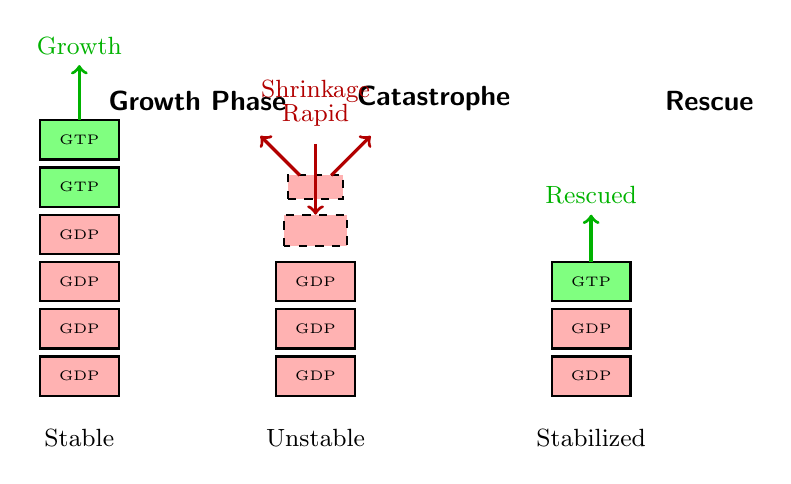
\begin{tikzpicture}[scale=1.0]
% Growth phase
\begin{scope}[shift={(0,0)}]
\node[above,font=\sffamily\bfseries] at (2,3.5) {Growth Phase};

% Microtubule body (GDP-tubulin)
\foreach \y in {0,0.6,1.2,1.8} {
    \draw[fill=red!30,draw=black,thick] (0,\y) rectangle (1,\y+0.5);
    \node[font=\tiny] at (0.5,\y+0.25) {GDP};
}

% GTP cap
\foreach \y in {2.4,3.0} {
    \draw[fill=green!50,draw=black,thick] (0,\y) rectangle (1,\y+0.5);
    \node[font=\tiny] at (0.5,\y+0.25) {GTP};
}

\draw[->,very thick,green!70!black] (0.5,3.5) -- (0.5,4.2) node[above,font=\small] {Growth};
\node[below,font=\small] at (0.5,-0.3) {Stable};
\end{scope}

% Catastrophe
\begin{scope}[shift={(3,0)}]
\node[above,font=\sffamily\bfseries] at (2,3.5) {Catastrophe};

% Microtubule body (GDP-tubulin) - shorter
\foreach \y in {0,0.6,1.2} {
    \draw[fill=red!30,draw=black,thick] (0,\y) rectangle (1,\y+0.5);
    \node[font=\tiny] at (0.5,\y+0.25) {GDP};
}

% Lost GTP cap - shown breaking apart
\draw[fill=red!30,draw=black,thick,dashed] (0.1,1.9) rectangle (0.9,2.3);
\draw[fill=red!30,draw=black,thick,dashed] (0.15,2.5) rectangle (0.85,2.8);

\draw[->,very thick,red!70!black] (0.5,3.2) -- (0.5,2.3);
\draw[->,very thick,red!70!black] (0.7,2.8) -- (1.2,3.3);
\draw[->,very thick,red!70!black] (0.3,2.8) -- (-0.2,3.3);
\node[above,font=\small,red!70!black] at (0.5,3.3) {Rapid};
\node[above,font=\small,red!70!black] at (0.5,3.6) {Shrinkage};
\node[below,font=\small] at (0.5,-0.3) {Unstable};
\end{scope}

% Rescue
\begin{scope}[shift={(6.5,0)}]
\node[above,font=\sffamily\bfseries] at (2,3.5) {Rescue};

% Microtubule body
\foreach \y in {0,0.6} {
    \draw[fill=red!30,draw=black,thick] (0,\y) rectangle (1,\y+0.5);
    \node[font=\tiny] at (0.5,\y+0.25) {GDP};
}

% New GTP cap forming
\draw[fill=green!50,draw=black,thick] (0,1.2) rectangle (1,1.7);
\node[font=\tiny] at (0.5,1.45) {GTP};

\draw[->,very thick,green!70!black] (0.5,1.7) -- (0.5,2.3) node[above,font=\small] {Rescued};
\node[below,font=\small] at (0.5,-0.3) {Stabilized};
\end{scope}
\end{tikzpicture}
\end{center}

\textbf{Kinetic parameters} (in vitro, 37$^\circ$C):

\begin{equation}
v_{\text{growth}} \approx 2~\mu\text{m/min}, \quad v_{\text{shrink}} \approx 10\text{--}20~\mu\text{m/min}
\label{eq:growth-shrink-rates}
\end{equation}

\begin{equation}
f_{\text{cat}} \approx 0.01~\text{s}^{-1}, \quad f_{\text{res}} \approx 0.001~\text{s}^{-1}
\label{eq:catastrophe-rescue-freq}
\end{equation}

where $f_{\text{cat}}$ is the catastrophe frequency and $f_{\text{res}}$ is the rescue frequency.

\begin{calloutbox}{Biological Function}
Dynamic instability enables rapid reorganization of the cytoskeleton during mitosis, cell migration, and axon guidance. The stochastic switching between growth and shrinkage allows cells to ``search'' space efficiently, a process critical for spindle assembly and neuronal pathfinding.
\end{calloutbox}

\section{Cellular Functions (Established)}
\label{sec:cellular-functions}

\subsection{Structural Support}
\label{subsec:structural-support}

\textbf{Mechanical properties}:
\begin{itemize}
\item \textbf{Young's modulus}: $\sim$1--2~GPa (stiffer than actin filaments)
\item \textbf{Persistence length}: $\sim$5~mm (very rigid on cellular scales)
\item \textbf{Buckling force}: $\sim$5~pN (can support compressive loads)
\end{itemize}

\textbf{Function}: Provide mechanical support and maintain cell shape. Microtubules resist compression and buckling, forming a rigid scaffold that organizes intracellular space.

\subsection{Intracellular Transport}
\label{subsec:intracellular-transport}

\textbf{Function}: Serve as tracks for motor protein-driven cargo transport.

\begin{center}
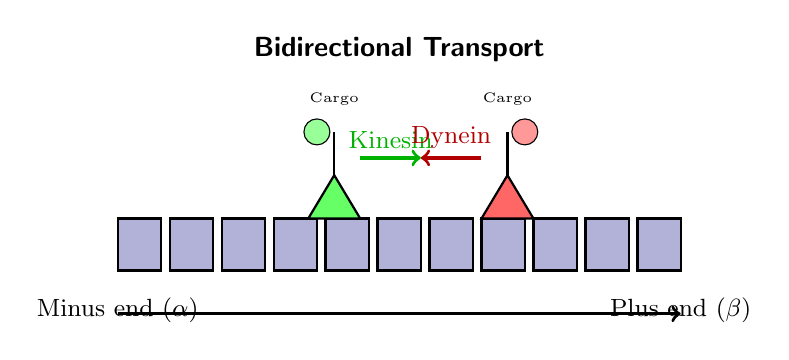
\begin{tikzpicture}[scale=1.1]
% Draw microtubule
\foreach \x in {0,0.6,1.2,1.8,2.4,3.0,3.6,4.2,4.8,5.4,6.0} {
    \draw[fill=NavyBlue!30,draw=black,thick] (\x,-0.3) rectangle (\x+0.5,0.3);
}

% Draw kinesin moving right (toward plus end)
\draw[fill=green!60,draw=black,thick] (2.2,0.3) -- (2.5,0.8) -- (2.8,0.3) -- cycle;
\draw[thick] (2.5,0.8) -- (2.5,1.3);
\draw[fill=green!40,draw=black] (2.3,1.3) circle (0.15);
\node[above,font=\tiny] at (2.5,1.5) {Cargo};
\draw[->,very thick,green!70!black] (2.8,1.0) -- (3.5,1.0);
\node[above,font=\small,green!70!black] at (3.15,1.0) {Kinesin};

% Draw dynein moving left (toward minus end)
\draw[fill=red!60,draw=black,thick] (4.8,0.3) -- (4.5,0.8) -- (4.2,0.3) -- cycle;
\draw[thick] (4.5,0.8) -- (4.5,1.3);
\draw[fill=red!40,draw=black] (4.7,1.3) circle (0.15);
\node[above,font=\tiny] at (4.5,1.5) {Cargo};
\draw[->,very thick,red!70!black] (4.2,1.0) -- (3.5,1.0);
\node[above,font=\small,red!70!black] at (3.85,1.0) {Dynein};

% Label microtubule polarity
\node[below,font=\small] at (0,-0.5) {Minus end ($\alpha$)};
\node[below,font=\small] at (6.5,-0.5) {Plus end ($\beta$)};
\draw[->,very thick] (0,-0.8) -- (6.5,-0.8);

\node[above,font=\sffamily\bfseries] at (3.25,2.0) {Bidirectional Transport};
\end{tikzpicture}
\end{center}

\textbf{Motor proteins}:
\begin{itemize}
\item \textbf{Kinesin}: Moves cargo toward plus end (cell periphery)
\item \textbf{Dynein}: Moves cargo toward minus end (cell center)
\item \textbf{Velocity}: $\sim$1~$\mu$m/s
\item \textbf{Force}: 5--7~pN per motor
\end{itemize}

\textbf{Medical relevance}: Defects in axonal transport linked to neurodegenerative diseases (Alzheimer's, ALS).

\subsection{Mitotic Spindle}
\label{subsec:mitotic-spindle}

\textbf{Function}: Segregate chromosomes during cell division with high fidelity.

\textbf{Structure}:
\begin{itemize}
\item \textbf{Astral microtubules}: Extend from centrosomes to cell cortex
\item \textbf{Kinetochore microtubules}: Attach to chromosomes
\item \textbf{Interpolar microtubules}: Overlap at spindle midzone
\end{itemize}

\textbf{Force generation}:
\begin{equation}
F_{\mathrm{chrom}} \approx 10~\mathrm{pN}
\end{equation}
where $F_{\mathrm{chrom}}$ is the force exerted on each chromosome by depolymerizing kinetochore microtubules.

\subsection{Cilia and Flagella}
\label{subsec:cilia-flagella}

\textbf{Structure}: \textbf{9+2 axoneme} (9 doublet microtubules + 2 central singlets)
\begin{itemize}
\item Dynein arms on doublets cause sliding $\rightarrow$ bending motion
\item Beat frequency: $\sim$10--60~Hz
\end{itemize}

\textbf{Examples}:
\begin{itemize}
\item \textbf{Respiratory cilia}: Clear mucus from airways
\item \textbf{Sperm flagella}: Propulsion
\item \textbf{Nodal cilia}: Establish left-right asymmetry in embryos
\end{itemize}


\section{Neural Microtubules: Unique Features}
\label{sec:neural-microtubules}

\subsection{Neuronal Cytoskeleton Organization}
\label{subsec:neuronal-cytoskeleton}

\textbf{Axons}:
\begin{itemize}
\item Microtubules uniformly oriented (plus-ends distal)
\item Continuous tracks for kinesin transport
\item Stabilized by tau protein (hyperphosphorylation in Alzheimer's)
\end{itemize}

\textbf{Dendrites}:
\begin{itemize}
\item Mixed polarity microtubules
\item Both kinesin and dynein active
\item Dynamic remodeling during synaptic plasticity
\end{itemize}

\textbf{Density}: $\sim$10$^{6}$ microtubules per neuron

\subsection{Post-Translational Modifications (PTMs)}
\label{subsec:ptms}

\textbf{Tubulin code}: $\sim$20 different PTMs create functional diversity.

\textbf{Key modifications}:
\begin{itemize}
\item \textbf{Acetylation} (Lys-40 on $\alpha$-tubulin): Marks stable, long-lived microtubules
\item \textbf{Tyrosination/detyrosination}: Regulates motor protein binding
\item \textbf{Polyglutamylation}: C-terminal tail modification (affects MAP binding)
\item \textbf{Phosphorylation}: Tau phosphorylation regulates microtubule stability
\end{itemize}

\subsection{Microtubule-Associated Proteins (MAPs)}
\label{subsec:maps}

\textbf{Examples}:
\begin{itemize}
\item \textbf{Tau}: Stabilizes microtubules (predominantly in axons)
\item \textbf{MAP2}: Stabilizes microtubules (predominantly in dendrites)
\item \textbf{MAP4}: Ubiquitous stabilizer
\item \textbf{EB proteins}: Track plus-ends (regulate dynamics)
\end{itemize}

\textbf{Anesthetic sensitivity}: General anesthetics (isoflurane, propofol) bind to tubulin and disrupt MAP interactions $\rightarrow$ altered microtubule dynamics.

\section{Quantum Hypotheses (Speculative)}
\label{sec:quantum-hypotheses}

\begin{warningbox}
The theories in this section are \textbf{highly speculative} and lack experimental confirmation. They are presented for completeness and to motivate future experimental tests, not as established science.
\end{warningbox}

\subsection{Orch-OR Theory (Penrose-Hameroff)}
\label{subsec:orch-or}

\textbf{Hypothesis}: Microtubules perform quantum computations beyond classical neuron networks, with consciousness arising from orchestrated objective reduction of quantum states.

\textbf{Status}: No experimental confirmation; decoherence time estimates vary wildly ($10^{-13}$~s to milliseconds).

\textbf{Proposed mechanism}:
\begin{enumerate}
\item Tubulin dimers exist in superposed states (conformational or electronic)
\item Quantum coherence spreads across $N = 10^{5}$--$10^{7}$ tubulins via dipole-dipole interactions
\item Superposition reaches OR threshold given by the Penrose criterion:
\begin{equation}
E \cdot \tau \sim \hbar
\end{equation}
where:
\begin{itemize}
\item $E$ = gravitationally induced self-energy difference between superposed states
\item $\tau$ = time until objective collapse
\item $\hbar = 1.055 \times 10^{-34}$~J$\cdot$s = reduced Planck constant
\end{itemize}
\item Wavefunction collapses $\rightarrow$ conscious moment ($\tau \sim 25$~ms, matching gamma oscillation period)
\end{enumerate}

\textbf{Requirements for viability}:
\begin{equation}
\tau_c > 1~\mathrm{ms}~\text{at}~T = 310~\mathrm{K}
\end{equation}
where:
\begin{itemize}
\item $\tau_c$ = coherence time
\item $T$ = physiological temperature
\item Isolation from environment (ordered water shell?)
\item Quantum-to-classical interface (how does OR generate neural firing?)
\end{itemize}

\subsection{Quantum Information Processing}
\label{subsec:quantum-computation}

\textbf{Hypothesis}: Microtubules perform quantum computations beyond classical neuron networks.

\textbf{Proposed qubit encoding schemes}:
\begin{itemize}
\item \textbf{Conformational qubits}: Tubulin dimer in superposition of two conformations
\item \textbf{Electronic qubits}: Aromatic amino acids in superposed $\pi$-electron states
\item \textbf{Phononic qubits}: THz vibrational modes (see Chapter~\ref{ch:thz-resonances})
\end{itemize}

\textbf{Entanglement propagation:}

Nearest-neighbor dipole coupling energy:
\begin{equation}
V_{ij} = \frac{\mu_i \cdot \mu_j}{4\pi\epsilon_0 r_{ij}^3} \sim 10^{-3}~\mathrm{eV}
\label{eq:dipole-coupling}
\end{equation}
where:
\begin{itemize}
\item $\mu_i, \mu_j$ = electric dipole moments of tubulins $i$ and $j$
\item $r_{ij} \approx 8$~nm = nearest-neighbor distance
\item $\epsilon_0$ = permittivity of free space
\end{itemize}

\textbf{Entanglement propagation}:

Nearest-neighbor dipole coupling energy:
\begin{equation}
V_{ij} = \frac{\mu_i \cdot \mu_j}{4\pi\epsilon_0 r_{ij}^3} \sim 10^{-3}~\mathrm{eV}
\label{eq:dipole-coupling}
\end{equation}
where:
\begin{itemize}
\item $\mu_i, \mu_j$ = electric dipole moments of tubulins $i$ and $j$
\item $r_{ij} \approx 8$~nm = nearest-neighbor distance
\item $\epsilon_0$ = permittivity of free space
\end{itemize}

\begin{center}
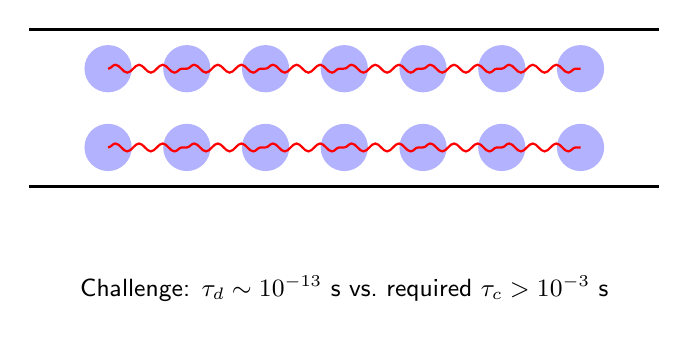
\begin{tikzpicture}[scale=1.0]
% Conceptual diagram of quantum coherence in microtubule
\draw[very thick] (-4,0) -- (4,0);
\draw[very thick] (-4,2) -- (4,2);

% Tubulin dimers as circles
\foreach \x in {-3,-2,-1,0,1,2,3} {
    \fill[blue!30] (\x,0.5) circle (0.3);
    \fill[blue!30] (\x,1.5) circle (0.3);
}

% Quantum coherence connections (wavy lines)
\foreach \x in {-3,-2,-1,0,1,2} {
    \draw[red,thick,decorate,decoration={snake,amplitude=0.5mm,segment length=3mm}] (\x,0.5) -- (\x+1,0.5);
    \draw[red,thick,decorate,decoration={snake,amplitude=0.5mm,segment length=3mm}] (\x,1.5) -- (\x+1,1.5);
}

% Decoherence representation
\node[below,font=\sffamily\small,align=center] at (0,-1) {Challenge: $\tau_d \sim 10^{-13}$ s vs.~required $\tau_c > 10^{-3}$ s};
\end{tikzpicture}
\end{center}

\textbf{Computational advantage}: Quantum parallelism $\rightarrow$ exponential speed-up for certain tasks (e.g., pattern recognition?)

\textbf{Problem}: No known biological algorithm requires quantum computation; classical neural networks already very powerful.

\subsection{Vibronic Coherence at Room Temperature}
\label{subsec:vibronic-coherence}

\textbf{Insight from VE-TFCC theory:} Strong vibronic coupling (electron-phonon interaction) can sustain thermal quantum coherence via Bogoliubov quasiparticles $\rightarrow$ stable coherent states at 310~K.

\textbf{Application to microtubules:} Aromatic residues (Trp, Tyr, Phe) have $\pi$-electron systems that couple to THz lattice vibrations $\rightarrow$ vibronic excitations.

\textbf{Coherence survival condition:}
\begin{equation}
g \omega \gtrsim k_B T
\end{equation}
where:
\begin{itemize}
\item $g$ = vibronic coupling constant
\item $\omega$ = phonon frequency (THz range)
\item $k_B T \approx 25$~meV at $T = 310$~K
\end{itemize}

For THz phonons at $\omega = 2\pi \times 1$~THz $= 4.1$~meV:
\begin{equation}
g_{\mathrm{required}} \gtrsim \frac{k_B T}{\omega} \approx 6
\end{equation}

\textbf{Testable prediction:} Measure quantum variance in microtubules:
\begin{equation}
\Delta q^2 = \langle q^2 \rangle - \langle q \rangle^2
\end{equation}
where excess variance (beyond classical thermal) indicates quantum coherence.

\textbf{Status:} Not yet measured experimentally

\section{Critical Challenges to Quantum Hypotheses}

\subsection{Decoherence Problem}

\textbf{Tegmark's calculation} (2000): Decoherence time in warm, wet brain environment:
\begin{equation}
\tau_d \sim \frac{\hbar}{E_{\mathrm{env}}} \sim 10^{-13}\ \mathrm{s}\ (100\ \mathrm{femtoseconds})
\end{equation}
where:
\begin{itemize}
\item $\tau_d$ = decoherence time
\item $E_{\mathrm{env}}$ = environmental interaction energy
\end{itemize}

\textbf{Dominant decoherence mechanisms:}
\begin{itemize}
\item Water dielectric fluctuations
\item Ion motion (Na$^+$, K$^+$, Ca$^{2+}$)
\item Thermal phonons ($k_B T \sim 25$~meV at 310~K)
\end{itemize}

\textbf{Decoherence rate estimate:}
\begin{equation}
\Gamma_{\mathrm{dec}} = \frac{1}{\tau_d} \sim 10^{13}\ \mathrm{s}^{-1}
\end{equation}

This is $10^{10}$ times faster than the required coherence time ($\tau_c > 1$~ms) for Orch-OR.

\textbf{Counter-arguments:}
\begin{itemize}
\item Tegmark assumed point dipoles; extended wavefunctions may decohere slower
\item Ordered water near microtubule surface reduces fluctuations
\item Vibronic coupling creates decoherence-free subspaces (VE-TFCC insight)
\end{itemize}

\textbf{Current status:} No consensus; experimental measurement needed

\subsection{Evolutionary Argument}
\label{subsec:evolutionary-argument}

\textbf{Critique}: If quantum effects were functionally important, we'd expect:
\begin{itemize}
\item Selection pressure to maintain coherence (e.g., specialized shielding proteins)
\item Deficits in organisms lacking microtubules (but prokaryotes have cognition without microtubules)
\end{itemize}

\textbf{Alternative explanation}: All known neural functions are explainable by classical electrophysiology.

\subsection{Anesthetic Paradox}
\label{subsec:anesthetic-paradox}

\textbf{Observation:} General anesthetics disrupt consciousness and bind to microtubules.

\textbf{Quantum interpretation:} Anesthetics disrupt THz coherence $\rightarrow$ loss of quantum computation $\rightarrow$ unconsciousness

\textbf{Classical interpretation:} Anesthetics alter microtubule-MAP interactions $\rightarrow$ disrupt synaptic vesicle transport $\rightarrow$ loss of neurotransmission

\textbf{Experimental test:} Does anesthetic binding shift THz resonances or reduce coherence times?
\begin{itemize}
\item \textbf{Preliminary data} (in vitro): Yes, small shifts ($\sim$0.1~THz)
\item \textbf{In vivo test}: Not yet done
\end{itemize}

\section{Worked Example: Microtubule Mechanical Analysis}

\textbf{Problem:} Calculate the force required to buckle a 10~$\mu$m microtubule segment under axial compression, and compare to typical cellular forces.

\subsection*{Given Parameters}

\begin{tabular}{@{}ll@{}}
Young's modulus & $E = 1.5$~GPa \\
Outer diameter & $D_{\mathrm{outer}} = 25$~nm \\
Inner diameter & $D_{\mathrm{inner}} = 15$~nm \\
Segment length & $L = 10$~$\mu$m \\
\end{tabular}

\subsection*{Step 1: Calculate Second Moment of Area}

For a hollow cylinder:
\begin{equation}
I = \frac{\pi}{64}(D_{\mathrm{outer}}^4 - D_{\mathrm{inner}}^4)
\end{equation}
\begin{equation}
I = \frac{\pi}{64}[(25 \times 10^{-9})^4 - (15 \times 10^{-9})^4] = 1.53 \times 10^{-32}\ \mathrm{m}^4
\end{equation}

\subsection*{Step 2: Calculate Buckling Force}

Using Euler's formula for a pinned-pinned column:
\begin{equation}
F_{\mathrm{buckle}} = \frac{\pi^2 EI}{L^2}
\end{equation}
\begin{equation}
F_{\mathrm{buckle}} = \frac{\pi^2 \times (1.5 \times 10^9) \times (1.53 \times 10^{-32})}{(10 \times 10^{-6})^2} = 2.26 \times 10^{-12}\ \mathrm{N} = 2.26\ \mathrm{pN}
\end{equation}

\subsection*{Step 3: Compare to Cellular Forces}

\begin{center}
\begin{tabular}{@{}lrl@{}}
\toprule
Force Source & \multicolumn{1}{c}{Force (pN)} & Comparison \\
\midrule
Kinesin motor & 5--7 & \textbf{Exceeds buckling force} \\
Dynein motor & 5--7 & \textbf{Exceeds buckling force} \\
Chromosome segregation & 10 & \textbf{4$\times$ buckling force} \\
Microtubule buckling & \textbf{2.3} & Baseline \\
\bottomrule
\end{tabular}
\end{center}

\subsection*{Conclusion}

The calculated buckling force ($\sim$2.3~pN) is \textbf{lower than typical cellular forces} (5--10~pN), meaning microtubules can buckle under compression from motor proteins or mitotic forces. This necessitates:
\begin{itemize}
\item Stabilization by MAPs (tau, MAP2) to increase effective stiffness
\item Crosslinking to adjacent microtubules to prevent buckling
\item Dynamic turnover to remove buckled microtubules
\end{itemize}

\subsection{Proposed Experiments}
\label{subsec:proposed-experiments}

\textbf{THz spectroscopy}:
\begin{itemize}
\item Two-dimensional THz on microtubules (detect off-diagonal coherences)
\item Temperature dependence (does coherence vanish classically at high $T$?)
\end{itemize}

\textbf{Isotope effects}:
\begin{itemize}
\item Deuterate tubulin (H $\rightarrow$ D changes vibrational frequencies)
\item Predict altered coherence times $\rightarrow$ test with cognitive assays
\end{itemize}

\textbf{Quantum sensors}:
\begin{itemize}
\item NV-diamond magnetometry: Detect weak magnetic fields from radical pairs in tubulin
\item SQUID arrays: Map magnetic coherence in brain slices
\end{itemize}


\section{Worked Example: Microtubule Depolymerization Force}
\label{sec:worked-example}

\textbf{Problem}: Calculate the maximum force a depolymerizing microtubule can exert on a chromosome during mitosis.

\subsection*{Given Parameters}

\begin{tabular}{@{}ll@{}}
Tubulin dimer size & $L = 8$~nm \\
Free energy of GTP hydrolysis & $\Delta G = 12$~k$_B$T per dimer \\
Temperature & $T = 310$~K (37$^\circ$C) \\
Boltzmann constant & $k_B = 1.38 \times 10^{-23}$~J/K \\
\end{tabular}

\subsection*{Step 1: Energy per Depolymerization Event}

The free energy released when one tubulin dimer dissociates:
\begin{equation}
\Delta G = 12 k_B T = 12 \times (1.38 \times 10^{-23}) \times 310 = 5.14 \times 10^{-20}~\text{J}
\label{eq:delta-g}
\end{equation}

\subsection*{Step 2: Maximum Force Calculation}

The maximum force occurs when all free energy is converted to mechanical work over the distance $L$:
\begin{equation}
F_{\text{max}} = \frac{\Delta G}{L} = \frac{5.14 \times 10^{-20}~\text{J}}{8 \times 10^{-9}~\text{m}} = 6.4 \times 10^{-12}~\text{N}
\label{eq:force-max}
\end{equation}

Converting to piconewtons:
\begin{equation}
F_{\text{max}} = 6.4~\text{pN}
\label{eq:force-pn}
\end{equation}

\subsection*{Step 3: Force per Protofilament}

For a 13-protofilament microtubule, if all protofilaments depolymerize simultaneously:
\begin{equation}
F_{\text{total}} = 13 \times F_{\text{max}} = 13 \times 6.4~\text{pN} = 83~\text{pN}
\label{eq:total-force}
\end{equation}

\begin{calloutbox}{Biological Significance}
\textbf{Result}: A single depolymerizing microtubule can exert $\sim$6--10~pN of force, sufficient to pull chromosomes during cell division. This force matches experimental measurements from laser trapping studies.

\textbf{Comparison}: This is comparable to forces generated by motor proteins (kinesin: 5--7~pN, dynein: 1--7~pN), demonstrating that depolymerization itself is a powerful force-generating mechanism.
\end{calloutbox}

\section{Applications}
\label{sec:applications}

\subsection{Drug Targets: Anti-Cancer Therapies}
\label{subsec:cancer-drugs}

\textbf{Microtubule-targeting agents (MTAs)} are among the most successful cancer chemotherapies.

\textbf{Mechanism}: Disrupting microtubule dynamics prevents cell division, selectively killing rapidly dividing cancer cells.

\textbf{Major drug classes}:

\begin{center}
\begin{tabular}{@{}lll@{}}
\toprule
\textbf{Drug} & \textbf{Mechanism} & \textbf{Clinical Use} \\
\midrule
Paclitaxel (Taxol) & Stabilizes microtubules & Breast, ovarian, lung cancer \\
Vinblastine & Inhibits polymerization & Hodgkin's lymphoma, testicular \\
Colchicine & Binds tubulin, prevents assembly & Gout (anti-inflammatory) \\
Docetaxel & Hyperstabilizes microtubules & Breast, prostate, gastric \\
\bottomrule
\end{tabular}
\end{center}

\textbf{Challenges}: Resistance develops through tubulin mutations or upregulation of drug efflux pumps (P-glycoprotein).

\subsection{Neurodegenerative Disease Biomarkers}
\label{subsec:neurodegen-biomarkers}

\textbf{Tau pathology}: Hyperphosphorylated tau detaches from microtubules $\rightarrow$ microtubule destabilization $\rightarrow$ impaired axonal transport $\rightarrow$ neuronal death.

\textbf{Diagnostic markers}:
\begin{itemize}
\item \textbf{CSF tau levels}: Elevated in Alzheimer's disease
\item \textbf{Tau PET imaging}: Visualizes neurofibrillary tangles in vivo
\item \textbf{Phospho-tau isoforms}: Differentiate Alzheimer's from other tauopathies
\end{itemize}

\textbf{Therapeutic strategies}:
\begin{itemize}
\item Tau aggregation inhibitors (e.g., methylthioninium)
\item Microtubule stabilizers (e.g., epothilone D, TPI-287)
\item Anti-tau antibodies (immunotherapy)
\end{itemize}

\subsection{Anesthesiology and Consciousness Research}
\label{subsec:anesthesia}

\textbf{Observation}: General anesthetics bind to hydrophobic pockets in tubulin at clinically relevant concentrations (EC$_{50}$ $\sim$ 0.1--1~mM).

\textbf{Binding sites}: Identified through X-ray crystallography and molecular dynamics
\begin{itemize}
\item Isoflurane: Binds between tubulin monomers
\item Propofol: Binds near GTP-binding pocket
\end{itemize}

\textbf{Functional effects}:
\begin{equation}
\text{Anesthetic binding} \rightarrow \text{Altered MT dynamics} \rightarrow \text{Disrupted vesicle transport?}
\label{eq:anesthetic-cascade}
\end{equation}

\begin{warningbox}
\textbf{Debate}: Whether anesthetic effects on microtubules are \textit{causal} for unconsciousness or \textit{correlational} remains unresolved. Most neuroscientists favor effects on ion channels and synaptic receptors as primary mechanisms.
\end{warningbox}

\subsection{Nanotechnology: Microtubules as Molecular Machines}
\label{subsec:nanotech}

\textbf{Biomimetic applications}:
\begin{itemize}
\item \textbf{Molecular railways}: Engineered kinesin motors on microtubule tracks for cargo sorting in lab-on-a-chip devices
\item \textbf{Nanoscale actuators}: Controlled polymerization/depolymerization for mechanical work
\item \textbf{Biosensors}: Microtubule-based detection of molecular binding events
\end{itemize}

\textbf{Example system}: Microtubule-based "smart dust" for environmental sensing
\begin{itemize}
\item Immobilize microtubules on microfluidic chips
\item Attach fluorescent cargo to kinesin motors
\item Measure transport velocity $\rightarrow$ reports on ATP concentration, temperature, or toxin presence
\end{itemize}

\section{See Also}
\label{sec:see-also}

\textbf{Related chapters on quantum effects in biological systems:}
\begin{itemize}
\item \textbf{Orchestrated Objective Reduction (Orch-OR)}: Consciousness theory requiring microtubule quantum effects
\item \textbf{Quantum Coherence in Biological Systems}: General framework for thermal quantum effects
\item \textbf{THz Resonances in Microtubules}: Vibrational modes that could sustain coherence
\item \textbf{Terahertz (THz) Technology}: Experimental probes for quantum measurements
\item \textbf{Hyper-Rotational Physics (HRP) Framework}: Theoretical extension to consciousness
\end{itemize}

\section{References}
\label{sec:references}

\textbf{Key references:}

\textit{Structure and Function (Established):}
\begin{enumerate}
\item \textbf{Nogales et al., \emph{Nature} 391, 199 (1998)} --- Tubulin crystal structure (foundational)
\item \textbf{Mitchison \& Kirschner, \emph{Nature} 312, 237 (1984)} --- Dynamic instability discovery
\item \textbf{Desai \& Mitchison, \emph{Annu. Rev.~Cell Dev. Biol.} 13, 83 (1997)} --- Microtubule dynamics review
\end{enumerate}

\textit{Quantum Hypotheses (Speculative):}
\begin{enumerate}
\setcounter{enumi}{3}
\item \textbf{Penrose \& Hameroff, \emph{Phys. Life Rev.} 11, 39 (2014)} --- Orch-OR consciousness theory
\item \textbf{Hameroff \& Penrose, \emph{J. Conscious. Stud.} 21, 126 (2014)} --- Orch-OR update
\end{enumerate}

\textit{Critical Perspectives:}
\begin{enumerate}
\setcounter{enumi}{5}
\item \textbf{Tegmark, \emph{Phys. Rev.~E} 61, 4194 (2000)} --- Decoherence calculation (skeptical)
\item \textbf{Koch \& Hepp, \emph{Nature} 440, 611 (2006)} --- Critique of quantum consciousness
\end{enumerate}

\textit{Vibronic Coupling:}
\begin{enumerate}
\setcounter{enumi}{7}
\item \textbf{Bao et al., \emph{J. Chem. Theory Comput.} 20, 4377 (2024)} --- VE-TFCC theory (thermal coherence)
\end{enumerate}

\textbf{Last updated}: October 2025
